% u1_poster/tex/teacher.tex — teacher key: the five group sheets with answers and finished graphs, plus scoring.
\documentclass[11pt]{article}
\usepackage{preamble}
\usepackage{amssymb}
\geometry{letterpaper,margin=0.6in}
% Key edition: collapse the student writing room so the key stays compact.
\renewcommand{\workspace}[1]{\par\vspace*{3pt}}
\newcommand{\sketchbox}[1]{}
\newcommand{\keygraph}[1]{\begin{callout}{\IconStar\ WHAT THE FINISHED GRAPH SHOULD LOOK LIKE}{calloutyellow}#1\end{callout}}
\begin{document}

\daybanner{AP Statistics \textperiodcentered\ Unit 1 Poster \textperiodcentered\ Teacher key}{Data, Graph, Sentence: five trio posters}

\begin{callout}{\IconBook\ HOW THE DAY RUNS}{calloutgreen}
\textbf{Groups of three.} Five groups, five sheets, every Unit 1 display covered: frequency table + bar chart (1), relative frequency table + relative frequency bar chart (2), dotplot (3), stem-and-leaf plot + histogram (4), parallel box plots (5). A pair takes sheet 3. Give the period's persistent misconception to a strong trio: \textbf{sheet 2 in Period B} (counts vs percents), \textbf{sheet 4 in Period E} (the mean is not resistant).\par\smallskip
\textbf{Order:} the trio solves (a)--(d) together on the sheet first. Then Data Keeper, Grapher and Writer split the poster. Every poster is Data, Graph, Sentence: the data table, the required display, and the DOK-3 answer in two or three sentences with numbers from the graph.\par\smallskip
\textbf{Two days are scheduled} (B: Thu 10/8 + Fri 10/9; E: Fri 10/9 + Wed 10/14). If a class finishes in one, run the gallery walk and start the Progress Check a day early.\par\smallskip
\textbf{Where the questions came from:} every claim on these sheets is a mistake this class made repeatedly on Unit 1 worksheets and quizzes, per the misconception tracker (215 flagged lines, 29 students): numbers without context, numeric labels treated as quantitative, counts compared across unequal groups, the mean treated as resistant, skew direction read backwards, SOCS descriptions missing unusual features, box plot sections misread as 75\%. The one Unit 1 cluster with no display behind it, z-scores read as percents, is left to the weekly DOK sheet.\par\smallskip
\textbf{Before handing out sheets:} project the example poster (separate PDF) and walk its Data, Graph, Sentence boxes with the talk-track on its page 2.
\end{callout}

\begin{callout}{\IconTarget\ SCORING (enter in Schoology, Posters category)}{calloutblue}
\begin{tabular}{p{0.45in}p{4.6in}p{0.7in}}
\textbf{E} & All five must-haves on the sheet's checklist. Display correctly drawn (scale, labels, units, key). Arithmetic right. Sentences in context with a number from the graph. & 100 \\[4pt]
\textbf{P} & Three or four must-haves, or all five with one error of direction or arithmetic (skew direction, a fence, a percent). & 85 \\[4pt]
\textbf{I} & Two or fewer must-haves, or the wrong kind of display for the data, or the answer agrees with the claim being judged. & 60 \\
\end{tabular}
\end{callout}

\begin{callout}{\IconSpeak\ DEBRIEF PROMPTS (10 minutes after the gallery walk)}{calloutyellow}
\begin{itemize}[leftmargin=1.4em,itemsep=2pt]
  \item Stand by the period's persistent poster (2 in B, 4 in E). ``This one came back after we taught it. What on this poster would have stopped it the second time?''
  \item ``Every poster's sentence has the same hidden rule. What is it?'' (A number means nothing without its variable, units and the question it answers.)
  \item Point at sheet 4 and sheet 3 together: ``Two different data sets, same lesson about the mean. Say it in one sentence.''
\end{itemize}
\end{callout}

\begin{center}\small
\begin{tabular}{|p{1.8in}|p{1.2in}|p{1.0in}|p{0.7in}|p{1.5in}|}\hline
\textbf{Poster} & \textbf{Group} & $\square\ \square\ \square\ \square\ \square$ & \textbf{E / P / I} & \textbf{Note} \\ \hline
1 Freq.\ table + bar chart & & & & \\[34pt] \hline
2 Rel.\ freq.\ table + chart & & & & \\[34pt] \hline
3 Dotplot & & & & \\[34pt] \hline
4 Stem-and-leaf + histogram & & & & \\[34pt] \hline
5 Parallel box plots & & & & \\[34pt] \hline
\end{tabular}
\end{center}

\newpage
% u1_poster/tex/cards.tex — shared content for the five Unit 1 poster group sheets.
% \answer{...} prints in the teacher edition only (student.tex redefines it to nothing).
% \keygraph{...} wraps the finished graph for the teacher key the same way.
%
% Every sheet is two pages:
%   page 1  data, the claim being judged, parts (a)-(d) with writing room
%   page 2  the poster checklist (= rubric), roles, a sketch box for the graph, a sentence frame + word bank

% Shared page-2 pieces -------------------------------------------------------
\newcommand{\posterrule}{All five $=$ E.\quad Three or four $=$ P.\quad Fewer $=$ I.}
\newcommand{\sketchtitle}[1]{\textbf{Sketch the graph here first.} #1\par\smallskip}
\newcommand{\draftline}{\par\medskip\textbf{Draft the poster sentences here.} Every sentence names the context and uses a number from the graph.}

% ============================================================================
% GROUP SHEET 1 — frequency table + bar chart
% ============================================================================
\ladderheading{AP Statistics \textperiodcentered\ Unit 1 Poster \textperiodcentered\ Group sheet 1 of 5}{Superpowers: Frequency Table + Bar Chart}

\focusbanner{YOUR POSTER SHOWS a frequency table AND a bar chart of the same data}

\textbf{Data (Lesson 1.3).} A random sample of 50 high school students was asked which superpower they would most like to have.

\begin{center}
\begin{tabular}{|l|c|c|c|c|c|}\hline
\textbf{Superpower} & Fly & Freeze time & Invisibility & Super strength & Telepathy \\ \hline
\textbf{Students} & 9 & 15 & 7 & 3 & 16 \\ \hline
\end{tabular}
\end{center}

\begin{callout}{\IconWarn\ THE CLAIM YOU ARE JUDGING}{calloutred}
A streaming service is pitching a show called \emph{Freeze Time}: \emph{``Freeze time is the superpower teens want most, and it is twice as popular as flying.''} A second writer says the show should be about telepathy.
\end{callout}

\dokbadge{1}~\textbf{(a)} Name the individuals and the variable. Is the variable categorical or quantitative? Why does that call for a bar chart instead of a dotplot or histogram?
\workspace{0.8in}
\answer{Individuals: the 50 students. Variable: preferred superpower, categorical (labels; averaging them is meaningless). Bar charts show counts or percents of categories; dotplots and histograms need a quantitative variable on the axis.}

\dokbadge{2}~\textbf{(b)} Check the pitch's two claims with the table. Is freeze time the \emph{most} chosen? Is it \emph{twice} as popular as flying? Show the numbers.
\workspace{0.95in}
\answer{Most: no. Telepathy 16 beats freeze time 15. Twice: no. $15 \div 9 \approx 1.7$; twice would be 18.}

\dokbadge{2}~\textbf{(c)} Write one claim about the two most popular superpowers that the data \emph{does} support. Include a number.
\workspace{0.8in}
\answer{$16 + 15 = 31$ of 50 students, $31/50 = 62\%$, chose telepathy or freeze time. Telepathy alone is 32\%, the single most popular choice.}

\dokbadge{3}~\textbf{(d)} $\star$ \textbf{For the poster:} in two or three sentences, say what the data supports, what it does not, and the honest claim. Name the context and use at least two numbers.
\workspace{1.45in}
\answer{Model: ``In a random sample of 50 high school students, telepathy was the most chosen superpower (16 students, 32\%), just ahead of freeze time (15, 30\%). Freeze time (15) was chosen more often than flying (9), but not twice as often. The honest pitch: 62\% of students chose either telepathy or freeze time.''}

\newpage
\begin{callout}{\IconTarget\ POSTER CHECKLIST \textperiodcentered\ Data \textperiodcentered\ Graph \textperiodcentered\ Sentence}{calloutblue}
\begin{itemize}[leftmargin=1.6em,itemsep=1pt,topsep=1pt]
  \item[$\square$] \textbf{Data:} the frequency table with a total row (adds to 50)
  \item[$\square$] \textbf{Graph:} bar chart: title, both axes labeled, bars separated, count scale that fits 16
  \item[$\square$] \textbf{Sentence:} individuals, variable, and ``categorical'' in one sentence
  \item[$\square$] \textbf{Sentence:} ``most'' and ``twice'' each judged with numbers
  \item[$\square$] \textbf{Sentence:} one honest claim, in context, with a number
\end{itemize}
\posterrule
\end{callout}

\begin{callout}{\IconPuzzle\ ROLES \textperiodcentered\ solve (a)--(d) together first, then split}{calloutgreen}
\textbf{Data Keeper:} table, total, the ``most'' / ``twice'' arithmetic.\quad
\textbf{Grapher:} the bar chart.\quad
\textbf{Writer:} the three sentences.
\end{callout}

\sketchbox{%
\sketchtitle{Bars separated, one per superpower.}
\begin{center}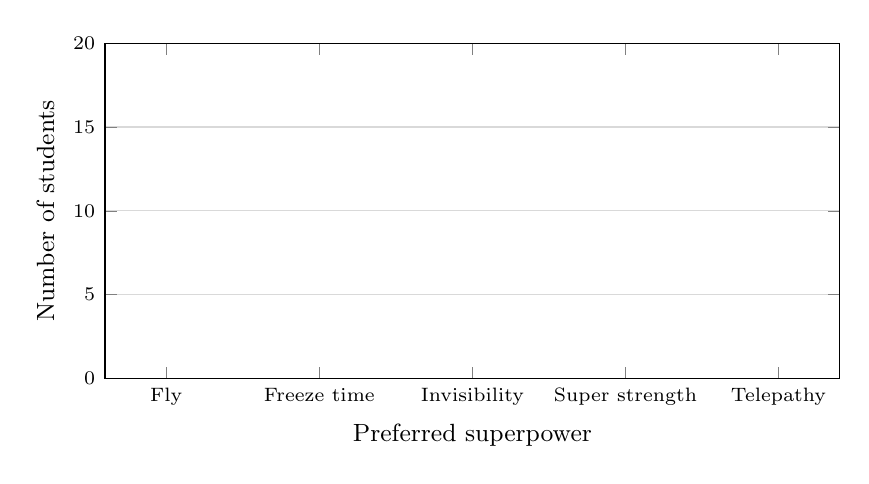
\begin{tikzpicture}
\begin{axis}[width=0.9\linewidth,height=2.3in,ymin=0,ymax=20,ytick={0,5,10,15,20},
 symbolic x coords={Fly,Freeze time,Invisibility,Super strength,Telepathy},xtick=data,
 xlabel={Preferred superpower},ylabel={Number of students},ymajorgrids,grid style={black!15},
 tick label style={font=\scriptsize},label style={font=\small}]
\addplot[draw=none,mark=none] coordinates {(Fly,0) (Freeze time,0) (Invisibility,0) (Super strength,0) (Telepathy,0)};
\end{axis}\end{tikzpicture}\end{center}
}

\begin{sentenceframebox}[top=3pt,bottom=3pt]\raggedright\textbf{Frame (optional):} In a sample of \blankt[0.5in]{how many} \blankt[0.9in]{who}, the most chosen superpower was \blankt[0.9in]{which}, with \blankt[0.4in]{count} students (\blankt[0.4in]{percent}). Freeze time was chosen about \blankt[0.7in]{how many times} as often as flying, so the pitch is \blankt[1.0in]{supported or not}.\end{sentenceframebox}

\begin{wordbankbox}[top=3pt,bottom=3pt]\small\raggedright
\textbf{Word bank:} telepathy \ensuremath{\;\cdot\;} freeze time \ensuremath{\;\cdot\;} 1.7 times \ensuremath{\;\cdot\;} twice \ensuremath{\;\cdot\;} 32\% \ensuremath{\;\cdot\;} 30\% \ensuremath{\;\cdot\;} 62\% \ensuremath{\;\cdot\;} not supported \ensuremath{\;\cdot\;} supported\quad {\footnotesize\color{framegray} Some words are not needed.}
\end{wordbankbox}

\draftline
\keygraph{%
\begin{center}\begin{tikzpicture}
\begin{axis}[ybar,bar width=22pt,width=0.8\linewidth,height=2.2in,ymin=0,ymax=20,ytick={0,5,10,15,20},
 symbolic x coords={Fly,Freeze time,Invisibility,Super strength,Telepathy},xtick=data,
 xlabel={Preferred superpower},ylabel={Number of students},title={Superpower preference, 50 students},
 tick label style={font=\scriptsize},label style={font=\small},title style={font=\small},nodes near coords,nodes near coords style={font=\scriptsize}]
\addplot[fill=calloutblue,draw=dayblue] coordinates {(Fly,9) (Freeze time,15) (Invisibility,7) (Super strength,3) (Telepathy,16)};
\end{axis}\end{tikzpicture}\end{center}}
\workspace{1.6in}

% ============================================================================
% GROUP SHEET 2 — relative frequency table + relative frequency bar chart
% ============================================================================
\newpage
\ladderheading{AP Statistics \textperiodcentered\ Unit 1 Poster \textperiodcentered\ Group sheet 2 of 5}{Spirit Day: Relative Frequency Table + Bar Chart}

\focusbanner{YOUR POSTER SHOWS a relative frequency table for both grades AND a side-by-side relative frequency bar chart}

\textbf{Data (Lesson 1.4).} A teacher surveyed two grades about their favorite spirit day theme.

\begin{center}
\begin{tabular}{|l|c|c|}\hline
\textbf{Theme} & \textbf{9th grade (30 students)} & \textbf{10th grade (20 students)} \\ \hline
Pajama Day & 12 & 5 \\ \hline
Jersey Day & 6 & 8 \\ \hline
Twin Day & 9 & 3 \\ \hline
Costume Day & 3 & 4 \\ \hline
\end{tabular}
\end{center}

\begin{callout}{\IconWarn\ THE CLAIM YOU ARE JUDGING}{calloutred}
Student council picked Jersey Day for the whole school: \emph{``Jersey Day got the most 10th-grade votes, and 9th grade was close anyway: 6 versus 8.''}
\end{callout}

\dokbadge{1}~\textbf{(a)} Turn every count into a percent of its own grade (divide by 30 or by 20). Check that each column totals 100\%.
\workspace{0.95in}
\answer{9th: Pajama 40\%, Jersey 20\%, Twin 30\%, Costume 10\%. 10th: Pajama 25\%, Jersey 40\%, Twin 15\%, Costume 20\%.}

\dokbadge{2}~\textbf{(b)} Which theme does each grade actually prefer? Is ``6 versus 8 is close'' still true in percents?
\workspace{1.35in}
\answer{9th prefers Pajama Day (40\%); 10th prefers Jersey Day (40\%). Jersey Day: 20\% of 9th graders vs 40\% of 10th graders, half as popular, not close. The counts only looked close because 9th grade has 30 students and 10th has 20.}

\dokbadge{2}~\textbf{(c)} In one or two sentences: why would a chart of raw counts have misled the council, and what does dividing by the group size fix?
\workspace{0.75in}
\answer{Counts can only be compared when groups are the same size; the 30-student grade looks more enthusiastic about everything. Dividing by group size puts both grades on the same 0 to 100\% scale.}

\dokbadge{3}~\textbf{(d)} $\star$ \textbf{For the poster:} the grades disagree. Recommend one schoolwide theme and defend it with percents in two or three sentences. Any theme is fine if the percents back it.
\workspace{0.85in}
\answer{Example: ``Pajama Day is the only theme chosen by at least a quarter of both grades (40\% of 9th graders, 25\% of 10th graders), so it is the fairest schoolwide pick. Jersey Day was 10th grade's favorite at 40\%, but only 20\% of 9th graders chose it. The council's `6 versus 8' compared counts from groups of 30 and 20, which is why it misled them.'' Jersey Day is acceptable if defended as ``10th grade's clear favorite at 40\%, and 9th grade's 20\% still beats Costume Day.''}

\newpage
\begin{callout}{\IconTarget\ POSTER CHECKLIST \textperiodcentered\ Data \textperiodcentered\ Graph \textperiodcentered\ Sentence}{calloutblue}
\begin{itemize}[leftmargin=1.6em,itemsep=1pt,topsep=1pt]
  \item[$\square$] \textbf{Data:} relative frequency table, eight percents, both columns total 100\%, two divisions shown
  \item[$\square$] \textbf{Graph:} side-by-side relative frequency bar chart: title, percent axis, key for the two grades
  \item[$\square$] \textbf{Sentence:} each grade's favorite, with its percent
  \item[$\square$] \textbf{Sentence:} ``6 versus 8 is close'' rejected with 20\% vs 40\%
  \item[$\square$] \textbf{Sentence:} the recommendation defended with percents, plus why counts mislead when groups differ in size
\end{itemize}
\posterrule
\end{callout}

\begin{callout}{\IconPuzzle\ ROLES \textperiodcentered\ solve (a)--(d) together first, then split}{calloutgreen}
\textbf{Data Keeper:} the eight percents and column totals.\quad
\textbf{Grapher:} the side-by-side chart with key.\quad
\textbf{Writer:} favorites, the recommendation, the ``why counts mislead'' sentence.
\end{callout}

\sketchbox{%
\sketchtitle{Two bars per theme, one shade per grade, with a key.}
\begin{center}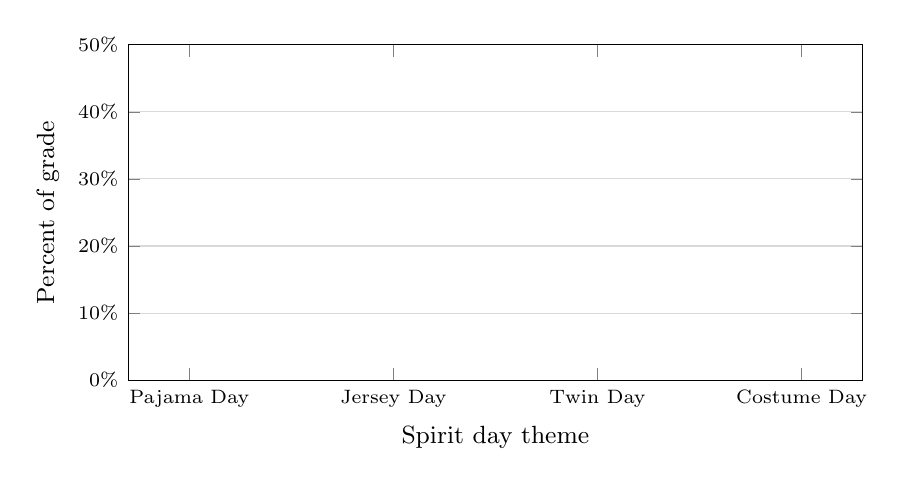
\begin{tikzpicture}
\begin{axis}[width=0.9\linewidth,height=2.3in,ymin=0,ymax=50,ytick={0,10,20,30,40,50},yticklabel={\pgfmathprintnumber{\tick}\%},
 symbolic x coords={Pajama Day,Jersey Day,Twin Day,Costume Day},xtick=data,
 xlabel={Spirit day theme},ylabel={Percent of grade},ymajorgrids,grid style={black!15},
 tick label style={font=\scriptsize},label style={font=\small}]
\addplot[draw=none,mark=none] coordinates {(Pajama Day,0) (Jersey Day,0) (Twin Day,0) (Costume Day,0)};
\end{axis}\end{tikzpicture}\end{center}
}

\begin{sentenceframebox}[top=3pt,bottom=3pt]\raggedright\textbf{Frame (optional):} Jersey Day was chosen by \blankt[0.5in]{percent} of 9th graders but \blankt[0.5in]{percent} of 10th graders, so the grades were \blankt[0.8in]{close or not}. The council compared \blankt[0.7in]{counts or percents} from groups of \blankt[0.35in]{size} and \blankt[0.35in]{size}, so \blankt[1.6in]{what went wrong}.\end{sentenceframebox}

\begin{wordbankbox}[top=3pt,bottom=3pt]\small\raggedright
\textbf{Word bank:} 20\% \ensuremath{\;\cdot\;} 40\% \ensuremath{\;\cdot\;} 25\% \ensuremath{\;\cdot\;} not close \ensuremath{\;\cdot\;} close \ensuremath{\;\cdot\;} counts \ensuremath{\;\cdot\;} percents \ensuremath{\;\cdot\;} 30 \ensuremath{\;\cdot\;} 20 \ensuremath{\;\cdot\;} the bigger grade looked more enthusiastic \ensuremath{\;\cdot\;} the smaller grade looked more enthusiastic\quad {\footnotesize\color{framegray} Some words are not needed.}
\end{wordbankbox}

\draftline
\keygraph{%
\begin{center}\begin{tikzpicture}
\begin{axis}[ybar,bar width=14pt,width=0.8\linewidth,height=2.2in,ymin=0,ymax=50,ytick={0,10,20,30,40,50},yticklabel={\pgfmathprintnumber{\tick}\%},
 symbolic x coords={Pajama Day,Jersey Day,Twin Day,Costume Day},xtick=data,
 xlabel={Spirit day theme},ylabel={Percent of grade},title={Favorite theme by grade},
 legend style={font=\scriptsize,at={(0.98,0.98)},anchor=north east},
 tick label style={font=\scriptsize},label style={font=\small},title style={font=\small}]
\addplot[fill=calloutblue,draw=dayblue] coordinates {(Pajama Day,40) (Jersey Day,20) (Twin Day,30) (Costume Day,10)};
\addplot[fill=calloutpeach,draw=warmred] coordinates {(Pajama Day,25) (Jersey Day,40) (Twin Day,15) (Costume Day,20)};
\legend{9th grade (30),10th grade (20)}
\end{axis}\end{tikzpicture}\end{center}}
\workspace{1.6in}

% ============================================================================
% GROUP SHEET 3 — dotplot
% ============================================================================
\newpage
\ladderheading{AP Statistics \textperiodcentered\ Unit 1 Poster \textperiodcentered\ Group sheet 3 of 5}{Late Bus: Dotplot}

\focusbanner{YOUR POSTER SHOWS a dotplot: every value as a dot on a number line with a scale}

\textbf{Data (Lesson 1.6).} A school recorded how many minutes 11 students waited for a late bus after school.

\begin{center}
\begin{tabular}{|l|c|c|c|c|c|c|c|c|c|c|c|}\hline
\textbf{Student} & 1 & 2 & 3 & 4 & 5 & 6 & 7 & 8 & 9 & 10 & 11 \\ \hline
\textbf{Minutes waiting} & 1 & 2 & 3 & 3 & 4 & 4 & 4 & 5 & 5 & 6 & 18 \\ \hline
\end{tabular}
\end{center}

\begin{callout}{\IconWarn\ THE CLAIM YOU ARE JUDGING}{calloutred}
The transportation office reports: \emph{``Students wait an average of 5 minutes for the late bus, so there is no problem.''}
\end{callout}

\dokbadge{1}~\textbf{(a)} Describe the distribution in context, one labeled line each: shape, center, variability, unusual features. (Sketch the dotplot on page 2 first if it helps.)
\workspace{0.95in}
\answer{Shape: skewed right, one peak at 4 minutes. Center: a typical wait is about 4 minutes (median 4). Variability: waits ran from 1 to 18 minutes. Unusual: a gap from 6 to 18 and one student at 18 minutes, an apparent outlier.}

\dokbadge{2}~\textbf{(b)} Find the five-number summary and the IQR. Is 18 an outlier by the $1.5 \times \text{IQR}$ rule? Show the fence.
\workspace{0.8in}
\answer{Min 1, Q1 3, median 4, Q3 5, max 18. IQR $= 5 - 3 = 2$. Upper fence $= 5 + 1.5(2) = 8$. 18 is above 8: an outlier.}

\dokbadge{2}~\textbf{(c)} The mean is $55 \div 11 = 5.0$ minutes and the median is 4. Which dot opens that gap? Which measure describes a typical wait, and why?
\workspace{0.75in}
\answer{The dot at 18 pulls the mean up: without it the other ten average $37/10 = 3.7$. The median stays at 4 because it depends on position only. The median describes the typical wait; the mean is not resistant to the outlier.}

\dokbadge{3}~\textbf{(d)} $\star$ \textbf{For the poster:} explain why ``average of 5, no problem'' hides the real problem, then rewrite the office's report honestly in one or two sentences, with numbers.
\workspace{1.3in}
\answer{Model: ``Most of the 11 students waited about 4 minutes for the late bus, but one student waited 18 minutes, far outside everyone else's 1 to 6 minutes. Averaging in that 18 produced the office's `5 minutes' and hid the real problem: one bus that was badly late.''}

\newpage
\begin{callout}{\IconTarget\ POSTER CHECKLIST \textperiodcentered\ Data \textperiodcentered\ Graph \textperiodcentered\ Sentence}{calloutblue}
\begin{itemize}[leftmargin=1.6em,itemsep=1pt,topsep=1pt]
  \item[$\square$] \textbf{Data:} the 11 values, the five-number summary, the IQR
  \item[$\square$] \textbf{Graph:} dotplot: 11 dots, number line 0 to 20 with even ticks, axis label with units, title
  \item[$\square$] \textbf{Sentence:} shape, center, variability, unusual features, each labeled and in context
  \item[$\square$] \textbf{Sentence:} the outlier check: Q1 3, Q3 5, IQR 2, fence $5 + 3 = 8$, so 18 is an outlier
  \item[$\square$] \textbf{Sentence:} the honest rewrite, with mean 5.0 vs median 4 explained from the dotplot
\end{itemize}
\posterrule
\end{callout}

\begin{callout}{\IconPuzzle\ ROLES \textperiodcentered\ solve (a)--(d) together first, then split}{calloutgreen}
\textbf{Data Keeper:} five-number summary, IQR, fence, mean.\quad
\textbf{Grapher:} the dotplot.\quad
\textbf{Writer:} the four description lines and the honest rewrite.
\end{callout}

\sketchbox{%
\sketchtitle{One dot per student; stack repeats.}
\begin{center}\begin{tikzpicture}[x=0.3in,y=0.2in]
\draw[->] (0,0) -- (20.8,0);
\foreach \x in {0,2,...,20} {\draw (\x,0.25) -- (\x,-0.25) node[below,font=\scriptsize] {\x};}
\foreach \x in {1,3,...,19} {\draw (\x,0.15) -- (\x,-0.15);}
\node[below=12pt,font=\small] at (10,0) {Minutes waiting for the late bus};
\path (0,4.5);
\end{tikzpicture}\end{center}
}

\begin{sentenceframebox}[top=3pt,bottom=3pt]\raggedright\textbf{Frame (optional):} The distribution of \blankt[1.3in]{variable in context} is \blankt[0.8in]{shape}, with a typical wait of about \blankt[0.35in]{number} minutes. Waits ranged from \blankt[0.3in]{min} to \blankt[0.3in]{max} minutes; \blankt[0.3in]{which value} is an outlier because it is above the fence of \blankt[0.3in]{fence}. The office's ``average of 5'' misleads because \blankt[1.7in]{reason}.\end{sentenceframebox}

\begin{wordbankbox}[top=3pt,bottom=3pt]\small\raggedright
\textbf{Word bank:} minutes waiting for the late bus \ensuremath{\;\cdot\;} skewed right \ensuremath{\;\cdot\;} skewed left \ensuremath{\;\cdot\;} symmetric \ensuremath{\;\cdot\;} 4 \ensuremath{\;\cdot\;} 5 \ensuremath{\;\cdot\;} 1 \ensuremath{\;\cdot\;} 18 \ensuremath{\;\cdot\;} 8 \ensuremath{\;\cdot\;} one long wait pulled the mean up \ensuremath{\;\cdot\;} the median is not resistant\quad {\footnotesize\color{framegray} Some words are not needed.}
\end{wordbankbox}

\draftline
\keygraph{%
\begin{center}\begin{tikzpicture}[x=0.28in,y=0.17in]
\draw[->] (0,0) -- (20.8,0);
\foreach \x in {0,2,...,20} {\draw (\x,0.25) -- (\x,-0.25) node[below,font=\scriptsize] {\x};}
\foreach \x/\y in {1/1,2/1,3/1,3/2,4/1,4/2,4/3,5/1,5/2,6/1,18/1} {\fill[dayblue] (\x,\y*1.0) circle (3.2pt);}
\node[below=12pt,font=\small] at (10,0) {Minutes waiting for the late bus};
\node[above,font=\small] at (10,4.2) {Late-bus wait times, 11 students};
\end{tikzpicture}\end{center}}
\workspace{1.6in}

% ============================================================================
% GROUP SHEET 4 — stem-and-leaf + histogram
% ============================================================================
\newpage
\ladderheading{AP Statistics \textperiodcentered\ Unit 1 Poster \textperiodcentered\ Group sheet 4 of 5}{Resting Heart Rate: Stem-and-Leaf Plot + Histogram}

\focusbanner{YOUR POSTER SHOWS a stem-and-leaf plot AND a histogram (bins of 5 bpm) of the same 25 values, side by side}

\textbf{Data (Lesson 1.2 spring-sport context).} Resting heart rate, in beats per minute (bpm), for 25 students who play a spring sport, already in order:

\begin{center}
{\small\texttt{42, 46, 50, 54, 57, 58, 59, 60, 60, 61, 62, 62, 62, 63, 64, 64, 65, 65, 66, 66, 67, 68, 68, 69, 70}}
\end{center}

\begin{callout}{\IconWarn\ THE CLAIM YOU ARE JUDGING}{calloutred}
The coach says: \emph{``Resting heart rate is skewed, so the mean is pulled up. I will use the mean as the typical athlete, and anyone below 50 bpm has to see the trainer.''}
\end{callout}

\dokbadge{1}~\textbf{(a)} Make the stem-and-leaf plot (stems 4 to 7, leaves in order, a key such as $6 \mid 2 = 62$ bpm). Tally the bins 40--44, 45--49, 50--54, 55--59, 60--64, 65--69, 70--74. Use the sketch boxes on page 2.
\workspace{1.25in}
\answer{$4 \mid 2\,6$;\ $5 \mid 0\,4\,7\,8\,9$;\ $6 \mid 0\,0\,1\,2\,2\,2\,3\,4\,4\,5\,5\,6\,6\,7\,8\,8\,9$;\ $7 \mid 0$. Bins: 1, 1, 2, 4, 9, 7, 1.}

\dokbadge{2}~\textbf{(b)} Shape: which way does the tail point? Which way does that pull the mean, above or below the median? Check with the actual mean (the 25 values sum to 1528) and the median.
\workspace{0.8in}
\answer{One peak in the 60s, tail toward the LOW values: skewed left. A left tail pulls the mean DOWN. Mean $= 1528/25 = 61.1$, median $= 62$ (13th value). The coach has the direction backwards.}

\dokbadge{2}~\textbf{(c)} Find Q1, Q3, the IQR and the lower fence. Which athletes are outliers by the $1.5 \times \text{IQR}$ rule? Does ``below 50'' match?
\workspace{0.6in}
\answer{Q1 $= (58+59)/2 = 58.5$ (median of the lower 12). Q3 $= (66+66)/2 = 66$. IQR $= 7.5$. Lower fence $= 58.5 - 1.5(7.5) = 47.25$. Outliers: 42 and 46. The 50 is not an outlier. The coach's cutoff happens to catch the same two athletes, but it was not derived from the data; the fence is 47.25.}

\dokbadge{3}~\textbf{(d)} $\star$ \textbf{For the poster:} in two or three sentences, which center should the coach report and why; and the trainer wants each athlete's exact number, so which display do you hand her and what does the other one hide?
\workspace{0.8in}
\answer{Model: ``Resting heart rates for the 25 athletes are skewed left with two low outliers (42 and 46 bpm), so the mean of 61.1 is pulled below the median of 62; the coach should report the median because it resists those outliers. Hand the trainer the stem-and-leaf plot: it shows every athlete's exact value, while the histogram groups them into 5-bpm bins and hides who is at 42 and 46.''}

\newpage
\begin{callout}{\IconTarget\ POSTER CHECKLIST \textperiodcentered\ Data \textperiodcentered\ Graph \textperiodcentered\ Sentence}{calloutblue}
\begin{itemize}[leftmargin=1.6em,itemsep=1pt,topsep=1pt]
  \item[$\square$] \textbf{Data:} the 25 values; mean 61.1, median 62, Q1 58.5, Q3 66, IQR 7.5, lower fence 47.25
  \item[$\square$] \textbf{Graph:} stem-and-leaf plot, stems 4--7, leaves in order, with a key
  \item[$\square$] \textbf{Graph:} histogram, bins 40--44 to 70--74, bars touching, axes labeled with units, title
  \item[$\square$] \textbf{Sentence:} ``skewed left'' with the tail direction, and mean vs median confirming it
  \item[$\square$] \textbf{Sentence:} which center to report and why; which display shows every athlete and what the histogram hides
\end{itemize}
\posterrule
\end{callout}

\begin{callout}{\IconPuzzle\ ROLES \textperiodcentered\ solve (a)--(d) together first, then split}{calloutgreen}
\textbf{Data Keeper:} mean, median, quartiles, fence, outliers.\quad
\textbf{Grapher:} both displays, side by side.\quad
\textbf{Writer:} shape and direction, the center choice, the trainer sentence.
\end{callout}

\sketchbox{%
\sketchtitle{Stem-and-leaf on the left, histogram on the right.}
\begin{center}
\begin{minipage}[c]{0.36\linewidth}\centering
\begin{tabular}{r|p{1.7in}}
\textbf{Stem} & \textbf{Leaf} \\ \hline
4 & \\[8pt]
5 & \\[8pt]
6 & \\[8pt]
7 & \\[8pt]
\end{tabular}\\[3pt]
{\scriptsize Key: \rule{0.4in}{0.4pt} $\mid$ \rule{0.3in}{0.4pt} $=$ \rule{0.5in}{0.4pt} bpm}
\end{minipage}\hfill
\begin{minipage}[c]{0.6\linewidth}\centering
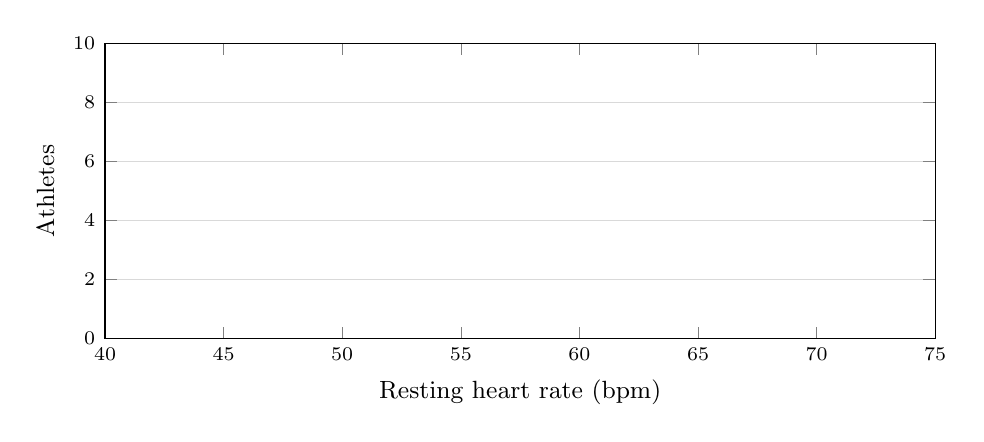
\begin{tikzpicture}
\begin{axis}[width=\linewidth,height=2.1in,xmin=40,xmax=75,ymin=0,ymax=10,
 xtick={40,45,...,75},ytick={0,2,4,6,8,10},xlabel={Resting heart rate (bpm)},ylabel={Athletes},
 ymajorgrids,grid style={black!15},tick label style={font=\scriptsize},label style={font=\small}]
\addplot[draw=none] coordinates {(40,0)};
\end{axis}\end{tikzpicture}
\end{minipage}
\end{center}
}

\begin{sentenceframebox}[top=3pt,bottom=3pt]\raggedright\textbf{Frame (optional):} The distribution of \blankt[1.3in]{variable in context} is skewed \blankt[0.45in]{direction}, so the mean of \blankt[0.4in]{value} is \blankt[0.5in]{above or below} the median of \blankt[0.35in]{value}. The coach should report the \blankt[0.55in]{which} because \blankt[1.3in]{reason}. The trainer gets the \blankt[1.0in]{which display} because \blankt[1.6in]{what the other hides}.\end{sentenceframebox}

\begin{wordbankbox}[top=3pt,bottom=3pt]\small\raggedright
\textbf{Word bank:} resting heart rate in bpm \ensuremath{\;\cdot\;} left \ensuremath{\;\cdot\;} right \ensuremath{\;\cdot\;} 61.1 \ensuremath{\;\cdot\;} 62 \ensuremath{\;\cdot\;} below \ensuremath{\;\cdot\;} above \ensuremath{\;\cdot\;} median \ensuremath{\;\cdot\;} mean \ensuremath{\;\cdot\;} it resists the two low outliers \ensuremath{\;\cdot\;} it follows the two low outliers \ensuremath{\;\cdot\;} stem-and-leaf plot \ensuremath{\;\cdot\;} histogram \ensuremath{\;\cdot\;} bins hide the exact values\quad {\footnotesize\color{framegray} Some words are not needed.}
\end{wordbankbox}

\draftline
\keygraph{%
\begin{center}
\begin{minipage}[c]{0.40\linewidth}\centering\footnotesize
\begin{tabular}{r|l}
\textbf{Stem} & \textbf{Leaf} \\ \hline
4 & 2 6 \\
5 & 0 4 7 8 9 \\
6 & 0 0 1 2 2 2 3 4 4 5 5 6 6 7 8 8 9 \\
7 & 0 \\
\end{tabular}\\[3pt]
{\scriptsize Key: $6 \mid 2 = 62$ bpm}
\end{minipage}\hfill
\begin{minipage}[c]{0.57\linewidth}\centering
\begin{tikzpicture}
\begin{axis}[width=\linewidth,height=2.1in,ybar interval,x tick label as interval=false,xmin=40,xmax=75,ymin=0,ymax=10,
 xtick={40,45,...,75},ytick={0,2,4,6,8,10},xlabel={Resting heart rate (beats per minute)},ylabel={Athletes},
 title={25 spring-sport athletes},tick label style={font=\scriptsize},label style={font=\small},title style={font=\small}]
\addplot[fill=calloutblue,draw=dayblue] coordinates {(40,1) (45,1) (50,2) (55,4) (60,9) (65,7) (70,1) (75,0)};
\end{axis}\end{tikzpicture}
\end{minipage}
\end{center}}
\workspace{1.2in}

% ============================================================================
% GROUP SHEET 5 — parallel box plots
% ============================================================================
\newpage
\ladderheading{AP Statistics \textperiodcentered\ Unit 1 Poster \textperiodcentered\ Group sheet 5 of 5}{Study Halls: Parallel Box Plots}

\focusbanner{YOUR POSTER SHOWS two box plots on ONE shared number line, the outlier as a separate point}

\textbf{Data (Lesson 1.9).} Nightly homework time, in minutes, for students in two study halls.

\begin{center}\small
\begin{tabular}{|l|c|c|c|c|c|c|}\hline
 & \textbf{Minimum} & \textbf{Q1} & \textbf{Median} & \textbf{Q3} & \textbf{Largest non-outlier} & \textbf{Outliers} \\ \hline
\textbf{Study Hall A} & 30 & 45 & 60 & 90 & 110 & one at 150 \\ \hline
\textbf{Study Hall B} & 45 & 54 & 60 & 66 & 75 (maximum) & none \\ \hline
\end{tabular}
\end{center}

\begin{callout}{\IconWarn\ THE CLAIMS YOU ARE JUDGING}{calloutred}
The principal: \emph{``Both study halls have a median of 60 minutes, so homework time is the same in both.''}\\
A parent: \emph{``What percent of Study Hall A students spent more than 90 minutes?''}
\end{callout}

\dokbadge{1}~\textbf{(a)} Sketch both box plots on the number line on page 2. Then find each study hall's IQR and range.
\workspace{0.7in}
\answer{A: IQR $= 90 - 45 = 45$; range $= 150 - 30 = 120$. B: IQR $= 66 - 54 = 12$; range $= 75 - 45 = 30$.}

\dokbadge{2}~\textbf{(b)} Compare the two: shape, center, variability, unusual features. Every line needs a comparative word (greater, less, similar, the same) and the context (homework minutes).
\workspace{0.95in}
\answer{Shape: A appears skewed right (long upper whisker, outlier); B appears roughly symmetric. Center: the median homework time is the same, 60 minutes. Variability: A's times are far more spread out (IQR 45 vs 12; range 120 vs 30). Unusual: A has one high outlier at 150 minutes; B has none.}

\dokbadge{2}~\textbf{(c)} Answer the parent. How does a box plot let you say that without the individual data?
\workspace{0.7in}
\answer{About 25\%: Q3 is 90, and each of the four sections of a box plot holds about one quarter of the data. (Above the median at 60 is 50\%, not 75\%.)}

\dokbadge{3}~\textbf{(d)} $\star$ \textbf{For the poster:} is the principal right? Use two features besides the median. Then: which study hall has the most predictable homework time, and which box-plot feature proves it? Two or three sentences.
\workspace{1.25in}
\answer{Model: ``The principal is wrong: the medians match at 60 minutes, but Study Hall A's times are far more spread out (IQR 45 vs 12 minutes, range 120 vs 30) and A has a 150-minute outlier while B has none. Study Hall B is more predictable: its narrower box and shorter whiskers mean the middle half of B's students finished within a 12-minute window.''}

\newpage
\begin{callout}{\IconTarget\ POSTER CHECKLIST \textperiodcentered\ Data \textperiodcentered\ Graph \textperiodcentered\ Sentence}{calloutblue}
\begin{itemize}[leftmargin=1.6em,itemsep=1pt,topsep=1pt]
  \item[$\square$] \textbf{Data:} both five-number summaries, both IQRs and ranges
  \item[$\square$] \textbf{Graph:} two box plots on one scale (30 to 150), labeled A and B, axis label with units, 150 as a separate point, each section labeled 25\%
  \item[$\square$] \textbf{Sentence:} four comparison lines (shape, center, variability, unusual), each with a comparative word, in context
  \item[$\square$] \textbf{Sentence:} the parent answered (about 25\%) with the ``each section is 25\%'' rule
  \item[$\square$] \textbf{Sentence:} the principal judged with numbers (IQR 45 vs 12, range 120 vs 30, outlier vs none) and the predictability pick tied to the narrower box
\end{itemize}
\posterrule
\end{callout}

\begin{callout}{\IconPuzzle\ ROLES \textperiodcentered\ solve (a)--(d) together first, then split}{calloutgreen}
\textbf{Data Keeper:} IQRs, ranges, the 25\% labels.\quad
\textbf{Grapher:} both plots on one scale, outlier as a point.\quad
\textbf{Writer:} four comparison lines, the parent's answer, the pick.
\end{callout}

\sketchbox{%
\sketchtitle{Study Hall A on the top row, B on the bottom, same number line.}
\begin{center}\begin{tikzpicture}[x=0.046in,y=0.22in]
\draw[->] (25,0) -- (158,0);
\foreach \x in {30,45,...,150} {\draw (\x,0.25) -- (\x,-0.25) node[below,font=\scriptsize] {\x};}
\node[below=12pt,font=\small] at (90,0) {Nightly homework time (minutes)};
\node[left,font=\small] at (26,2) {A};
\node[left,font=\small] at (26,4.5) {B};
\draw[black!20] (25,2) -- (158,2);
\draw[black!20] (25,4.5) -- (158,4.5);
\path (25,6);
\end{tikzpicture}\end{center}
}

\begin{sentenceframebox}[top=3pt,bottom=3pt]\raggedright\textbf{Frame (optional):} The median homework time is \blankt[0.7in]{comparative} for both study halls at \blankt[0.35in]{value} minutes, but Study Hall A's times are \blankt[0.7in]{comparative} spread out (IQR \blankt[0.3in]{value} vs \blankt[0.3in]{value} minutes) and A has \blankt[0.9in]{unusual feature}. About \blankt[0.35in]{percent} of A spent more than 90 minutes because \blankt[1.7in]{box plot rule}.\end{sentenceframebox}

\begin{wordbankbox}[top=3pt,bottom=3pt]\small\raggedright
\textbf{Word bank:} the same \ensuremath{\;\cdot\;} greater \ensuremath{\;\cdot\;} less \ensuremath{\;\cdot\;} far more \ensuremath{\;\cdot\;} 60 \ensuremath{\;\cdot\;} 45 \ensuremath{\;\cdot\;} 12 \ensuremath{\;\cdot\;} 25\% \ensuremath{\;\cdot\;} 50\% \ensuremath{\;\cdot\;} 75\% \ensuremath{\;\cdot\;} one high outlier at 150 \ensuremath{\;\cdot\;} no outliers \ensuremath{\;\cdot\;} each section of a box plot holds about a quarter of the data\quad {\footnotesize\color{framegray} Some words are not needed.}
\end{wordbankbox}

\draftline
\keygraph{%
\begin{center}\begin{tikzpicture}
\begin{axis}[width=0.85\linewidth,height=2.0in,xmin=20,xmax=160,xtick={30,45,60,75,90,105,120,135,150},
 ytick={1,2},yticklabels={Study Hall B,Study Hall A},ymin=0.4,ymax=2.6,xlabel={Nightly homework time (minutes)},
 title={Two study halls},tick label style={font=\scriptsize},label style={font=\small},title style={font=\small}]
\addplot+[boxplot prepared={lower whisker=45,lower quartile=54,median=60,upper quartile=66,upper whisker=75,draw position=1},fill=calloutpeach,draw=warmred,mark=none] coordinates {};
\addplot+[boxplot prepared={lower whisker=30,lower quartile=45,median=60,upper quartile=90,upper whisker=110,draw position=2},fill=calloutblue,draw=dayblue,mark=none] coordinates {};
\addplot[only marks,mark=*,mark size=2pt,dayblue] coordinates {(150,2)};
\end{axis}\end{tikzpicture}\end{center}}
\workspace{1.4in}

\end{document}
